\documentclass[
peprint,
amsmath,amssymb,
aip,
jap,
floatfix,
]{revtex4-2}

\usepackage{graphicx}
\usepackage{dcolumn}
\usepackage{bm}
\usepackage{siunitx}
\usepackage{xcolor, soul}
\usepackage{calc}
 % \usepackage{titling}
\definecolor{Red}{RGB}{163, 25, 25}
\usepackage{enumitem}
\usepackage{titlesec}
  \titleformat{\chapter}[display]
    {\normalfont\huge\bfseries}
    {\filcenter\underline}
    {\filcenter\underline{\MakeUppercase{\textls[400]{\chaptertitlename}}\ \thechapter}}{20pt}{\Huge}


  \titleformat{\section}
    {\bfseries\color{Red} \Large}
    {}
    {0em}
    {}[\titlerule]

  
  \titleformat{\subsection}
   {\bfseries\color{Red}}
   {}
   {0em}
   {}


  \titleformat{\subsubsection}[runin]
    {\bfseries}
    {}
    {0em}
    {}
  \titlespacing{\subsubsection}
    {0pt}
    {0.01in}
    {0.08in}
    {}

  \titlespacing{\subsection}
    {0pt}
    {0.05in}
    {0.05in}
  \titlespacing{\section}
    {0pt}
    {0.05in}
    {0.05in}

  \titleformat{\subsubsubsection} 
    {\bfseries}
    {}
    {0.1in}
    {}

\begin{document} 


  \title{An investigation of the coupling of phonon-polaritons with plasmon-polaritons in hBN/nanopatterned Au layered devices}
  \maketitle
  \section{Results and Discussion}
  \label{sec:RnD}
  	Electromagnetic simulations were performed using the Finite-Difference Time-Domain (FDTD) method \cite{Kane:66} using an in-house designed code. The FDTD method numerically integrates the Maxwell curl equations with second-order accuracy as detailed in Ref. \cite{Taflove:05}.

      \begin{figure}[!htb]
        \centering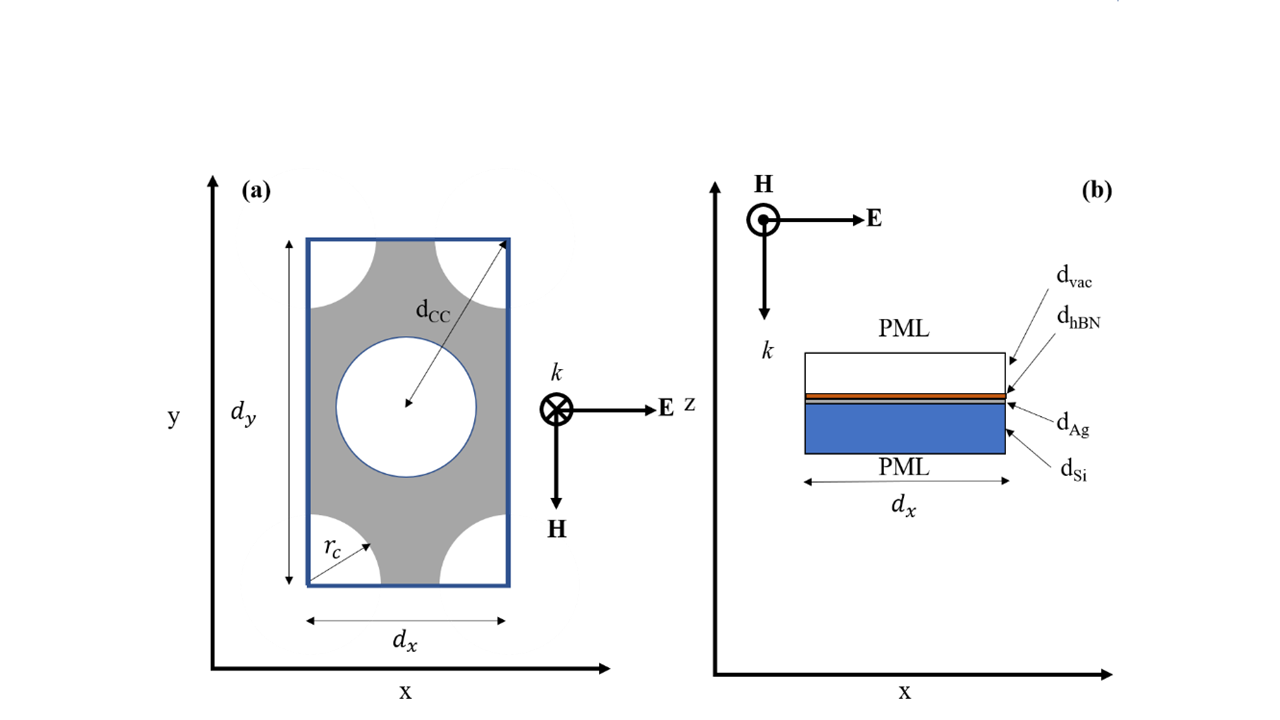
\includegraphics[width=0.9\textwidth]{FiguresCh4/StructurehBNAgHex.png}
        \caption{Schematic of the hBN/Ag structure simulated on this work. \textbf{(a)} Plane view at the hBN/Ag interface. The symmetry reduced unit cell is outlined in red. \textbf{(b)} Cross-sectional view. CPML: Convolutional perfectly matched layer boundary conditions terminated the z direction boundaries. Periodic boundary conditions terminated the x and y boundaries. The unit cell lengths in the x- and y- directions are $d_{x} $ and $d_{y}$, respectively. The layer thicknesses beyond the CPMLs were $d_{\rm{VAC}} = 0.87$ $\rm \mu$m, $d_{\rm{hBN}} = 80$ nm, $d_{\rm{Si}} = 1.0$ $\rm \mu$m, $d_{\rm{Ag}} = 50$ nm. The radius of the holes is $r_{C} = 0.68$ $\rm \mu$m. The distance between the centers of the cylindrical holes is $d_{CC} = d_{x} $. The directions of the \textbf{\textit{E}}-field, \textbf{\textit{H}}-Field and propagation vector \textbf{\textit{k}} is shown in both panes.}
        \label{fig:1}
      \end{figure}

    The details of the nanopatterned structure simulated in this work are shown in Figure ~\ref{fig:1}. The structure comprised of an 80 nm sheet of hexagonal boron nitride (hBN) deposited on a 50 nm thick film of nanopatterned Ag atop of a Si substrate. The Ag film was patterned with circular holes of radius 0.68 $\rm \mu m$ arranged in a hexagonal lattice with a distance between the centers of $\rm d_{CC}$, which was varied during this work.

    For all simulations performed a broadband, plane wave source was used. The time profile of the source was a Ricker wavelet \cite{Ricker:43} centered on 1667 $\rm cm^{-1} (6  \mu m$). This source injects a laterally uniform in time pulse using the total-field scattered-field (TFSF) interface \cite{Merewether:80}. The source was x-polarized and propagated in the negative z-direction. The use of the TFSF method enabled sensors to be placed above the TFSF boundary in order to record only the reflected field values.

      \begin{figure}[!htb]
        \centering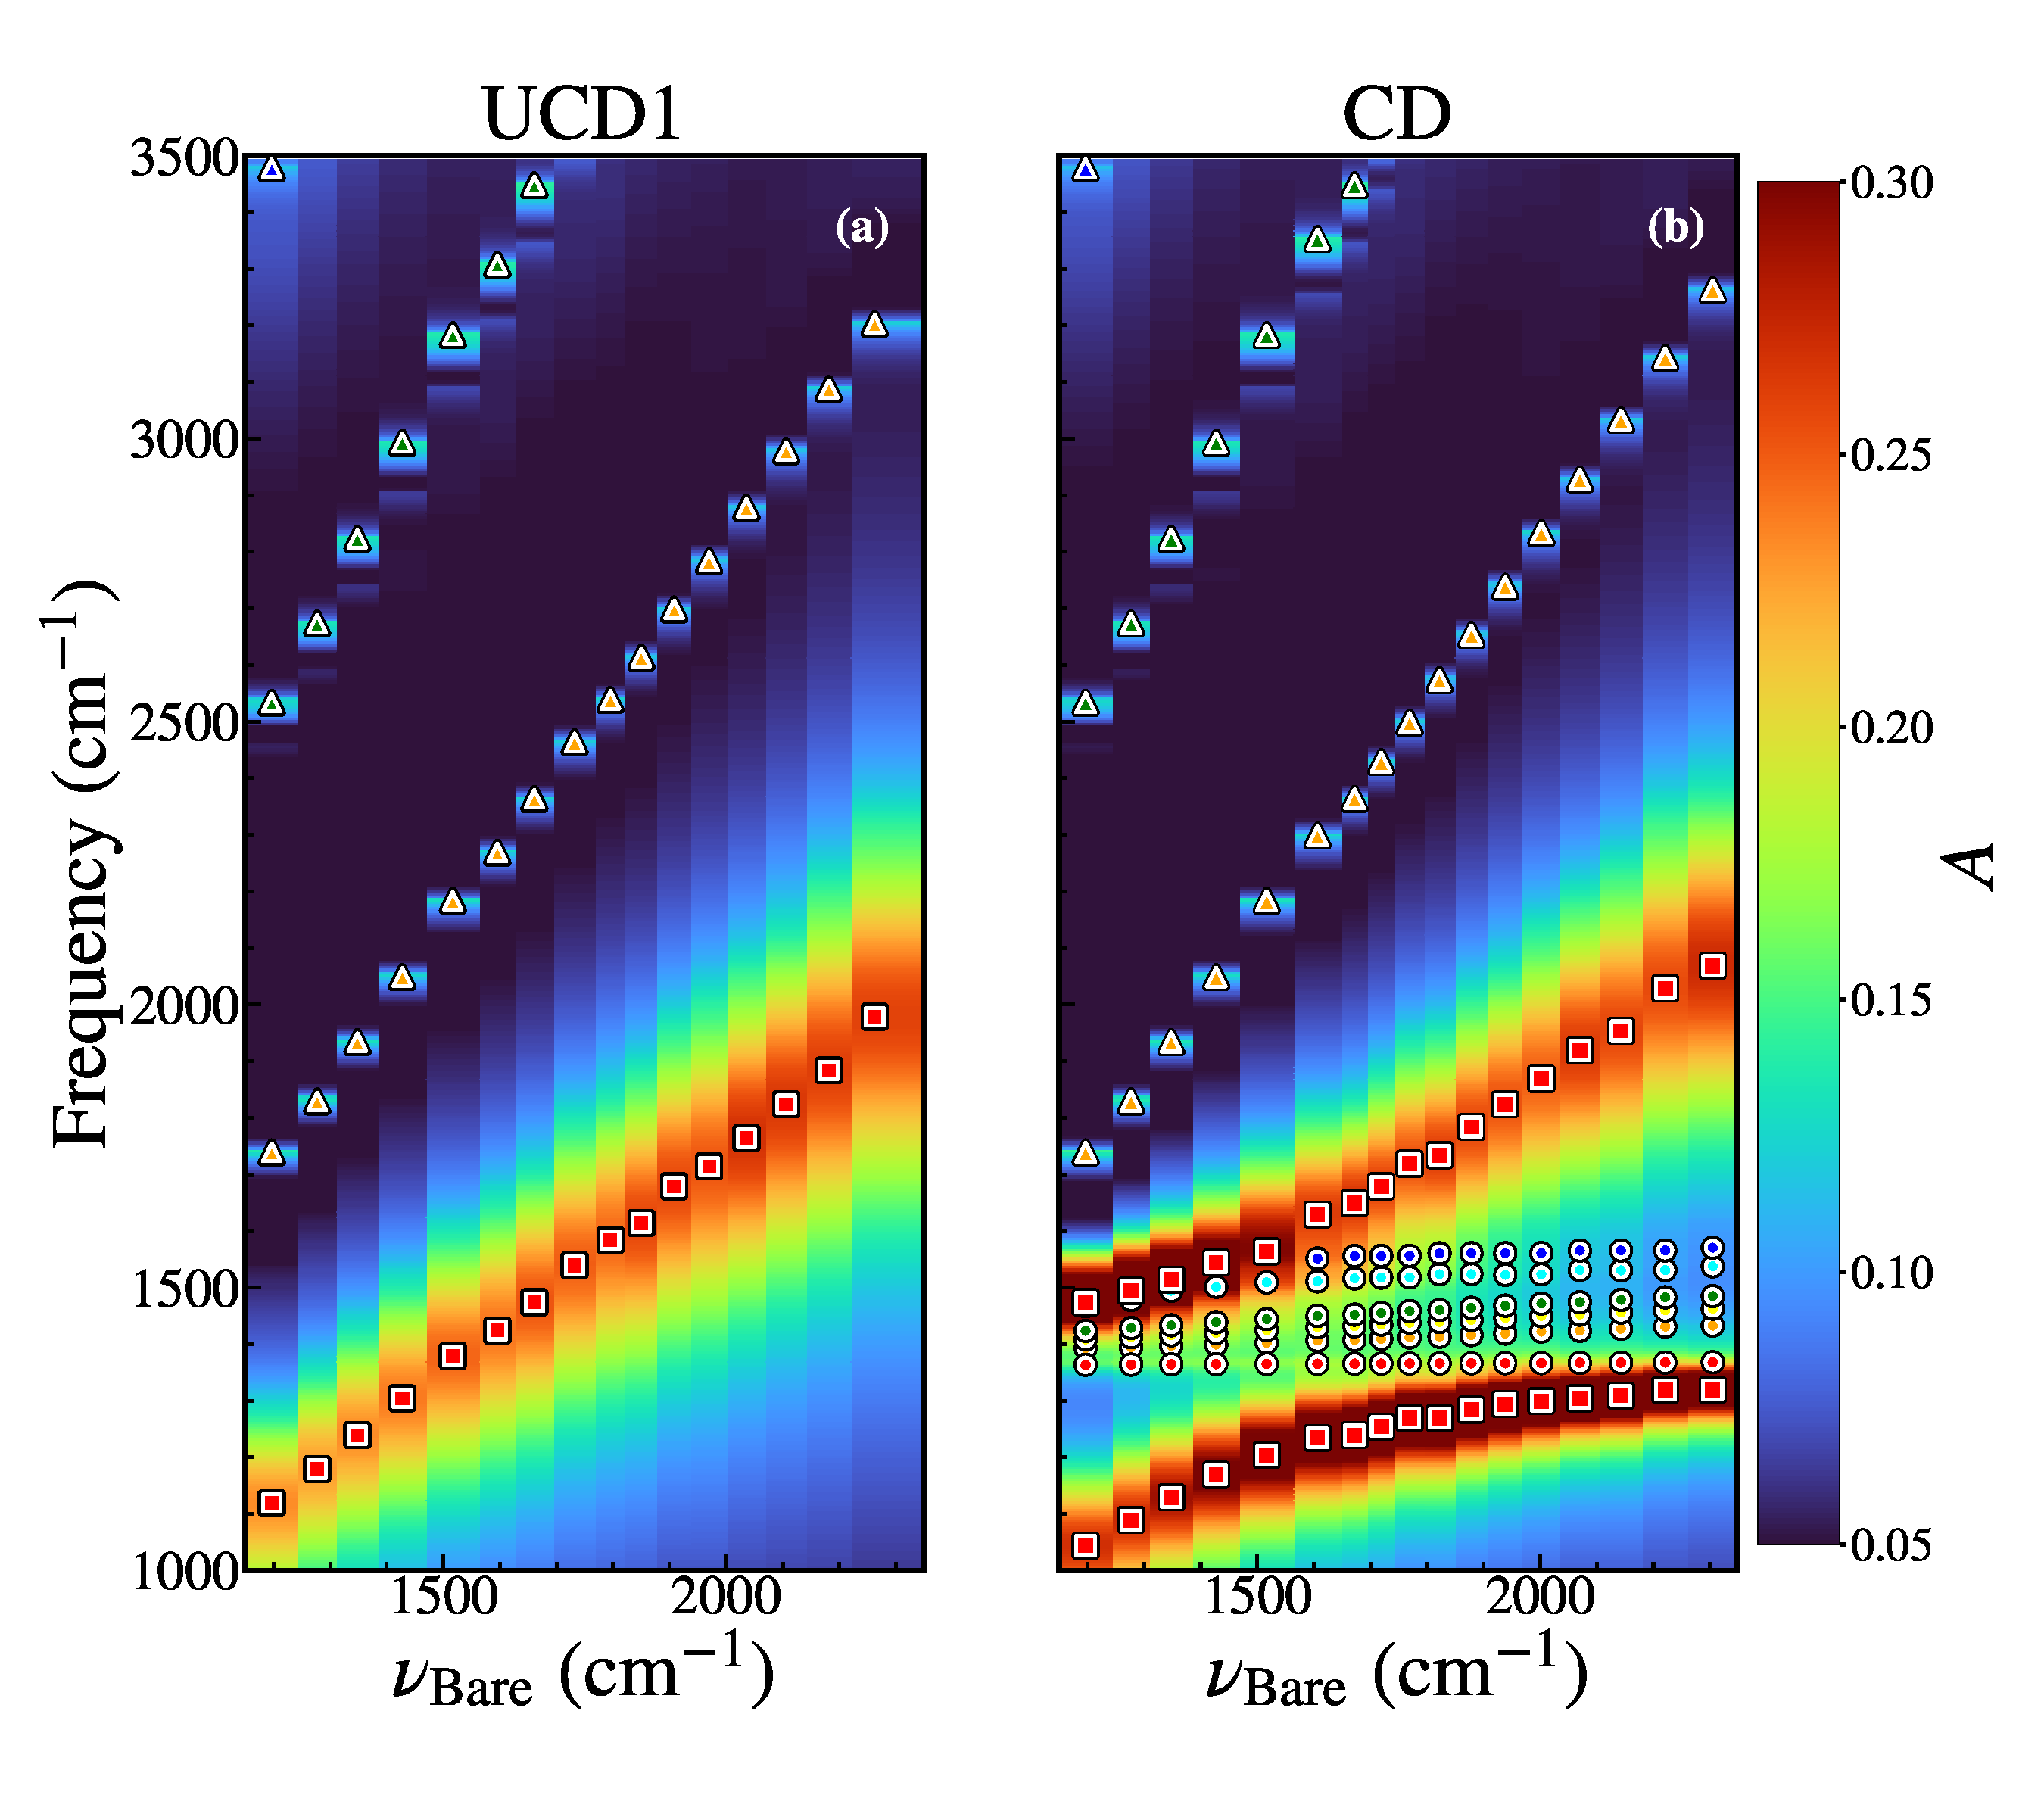
\includegraphics[width=0.5\textwidth]{Mar5DisserrtationPics/Fig3.png}
        \caption{\textbf{(a)} The absorptance spectrum of the bare nanopatterned Ag on Si device as function of $d_{CC}$. \textbf{(b)} The absorptance spectra of devices with an uncoupled anisotropic dielectric layer on top of the structures depicted in \textbf{(a)}. \textbf{(c)} The absorptance spectra of devices with an hBN (coupled) layer on structures depicted in \textbf{(a)}. The vertical black line in this figure indicates the absorption peak that was observed for the 80 nm thick layer of hBN in vacuum shown in Figure \textcolor{cyan}{ref{fig:2}}.}
        \label{fig:3}
      \end{figure}

    In order to ensure resonance between the polaritons supported by the hBN layer and the plasmons supported by the nanopatterned Ag/Si structure (bare device). A series of FDTD simulations were performed at range of distances between the centers of the holes ($d_{CC}$). The absorptance spectrum for each of the structures was calculated as described above. As the value of $d_{CC}$ was increased, a red shift in the absorptance spectrum was observed, as shown in Figure ~\ref{fig:3} (a). This observation enabled the absorptance resonance of the bare device to be tuned to close the resonance observed in Figure \textcolor{cyan}{ref{fig:2}} (c) for an 80 nm thick layer of hBN. Following the approach of Wan \textit{et al}. \cite{Wan:16}, the properties of a second series of devices (uncoupled devices) with a nonresonant dielectric layer on top of the nanopatterned Ag/Si structure (bare device) are also investigated. Specifically, for these devices, the top layer is an anisotropic dielectric with $\varepsilon_{x,y}(\infty)= \rm{4.87}$ and $\varepsilon_{z}(\infty)= \rm{2.95}$, respectively (i.e., $\varepsilon_{x,y}(\infty)$ and $\varepsilon_{z}(\infty)$ for hBN, respectively). The absorptance spectra for the uncoupled devices are shown in Figure ~\ref{fig:3} (b). The peaks of the uncoupled device absorptance spectra are slightly red-shifted compared to the peaks of the bare device absorption spectra. The uncoupled device with an absorptance peak that is most resonant with the hBN absorption peak is the device with $d_{CC}$ = 2.38 $\rm \mu$m. The final series of devices (coupled devices), comprising an 80 nm thick hBN layer on top of the bare devices. The absorptance of the coupled devices are shown in Figure  ~\ref{fig:3} (c). In this case the absorptance spectra splits into two major peaks, the positions of which vary with $d_{CC}$ or equivalently with the frequency ($\nu_{\rm{bare}}$) of the peak absorptance of the bare device. In addition, there is a smaller peak at 1468 $\rm cm^{-1}$ the position of which is independent of $d_{CC}(\nu_{\rm{bare}})$, it is notable that this peak occurs in the spectral region where Re $\varepsilon_{x,y}$ is strongly negative.


      \begin{figure}[!htb]
        \centering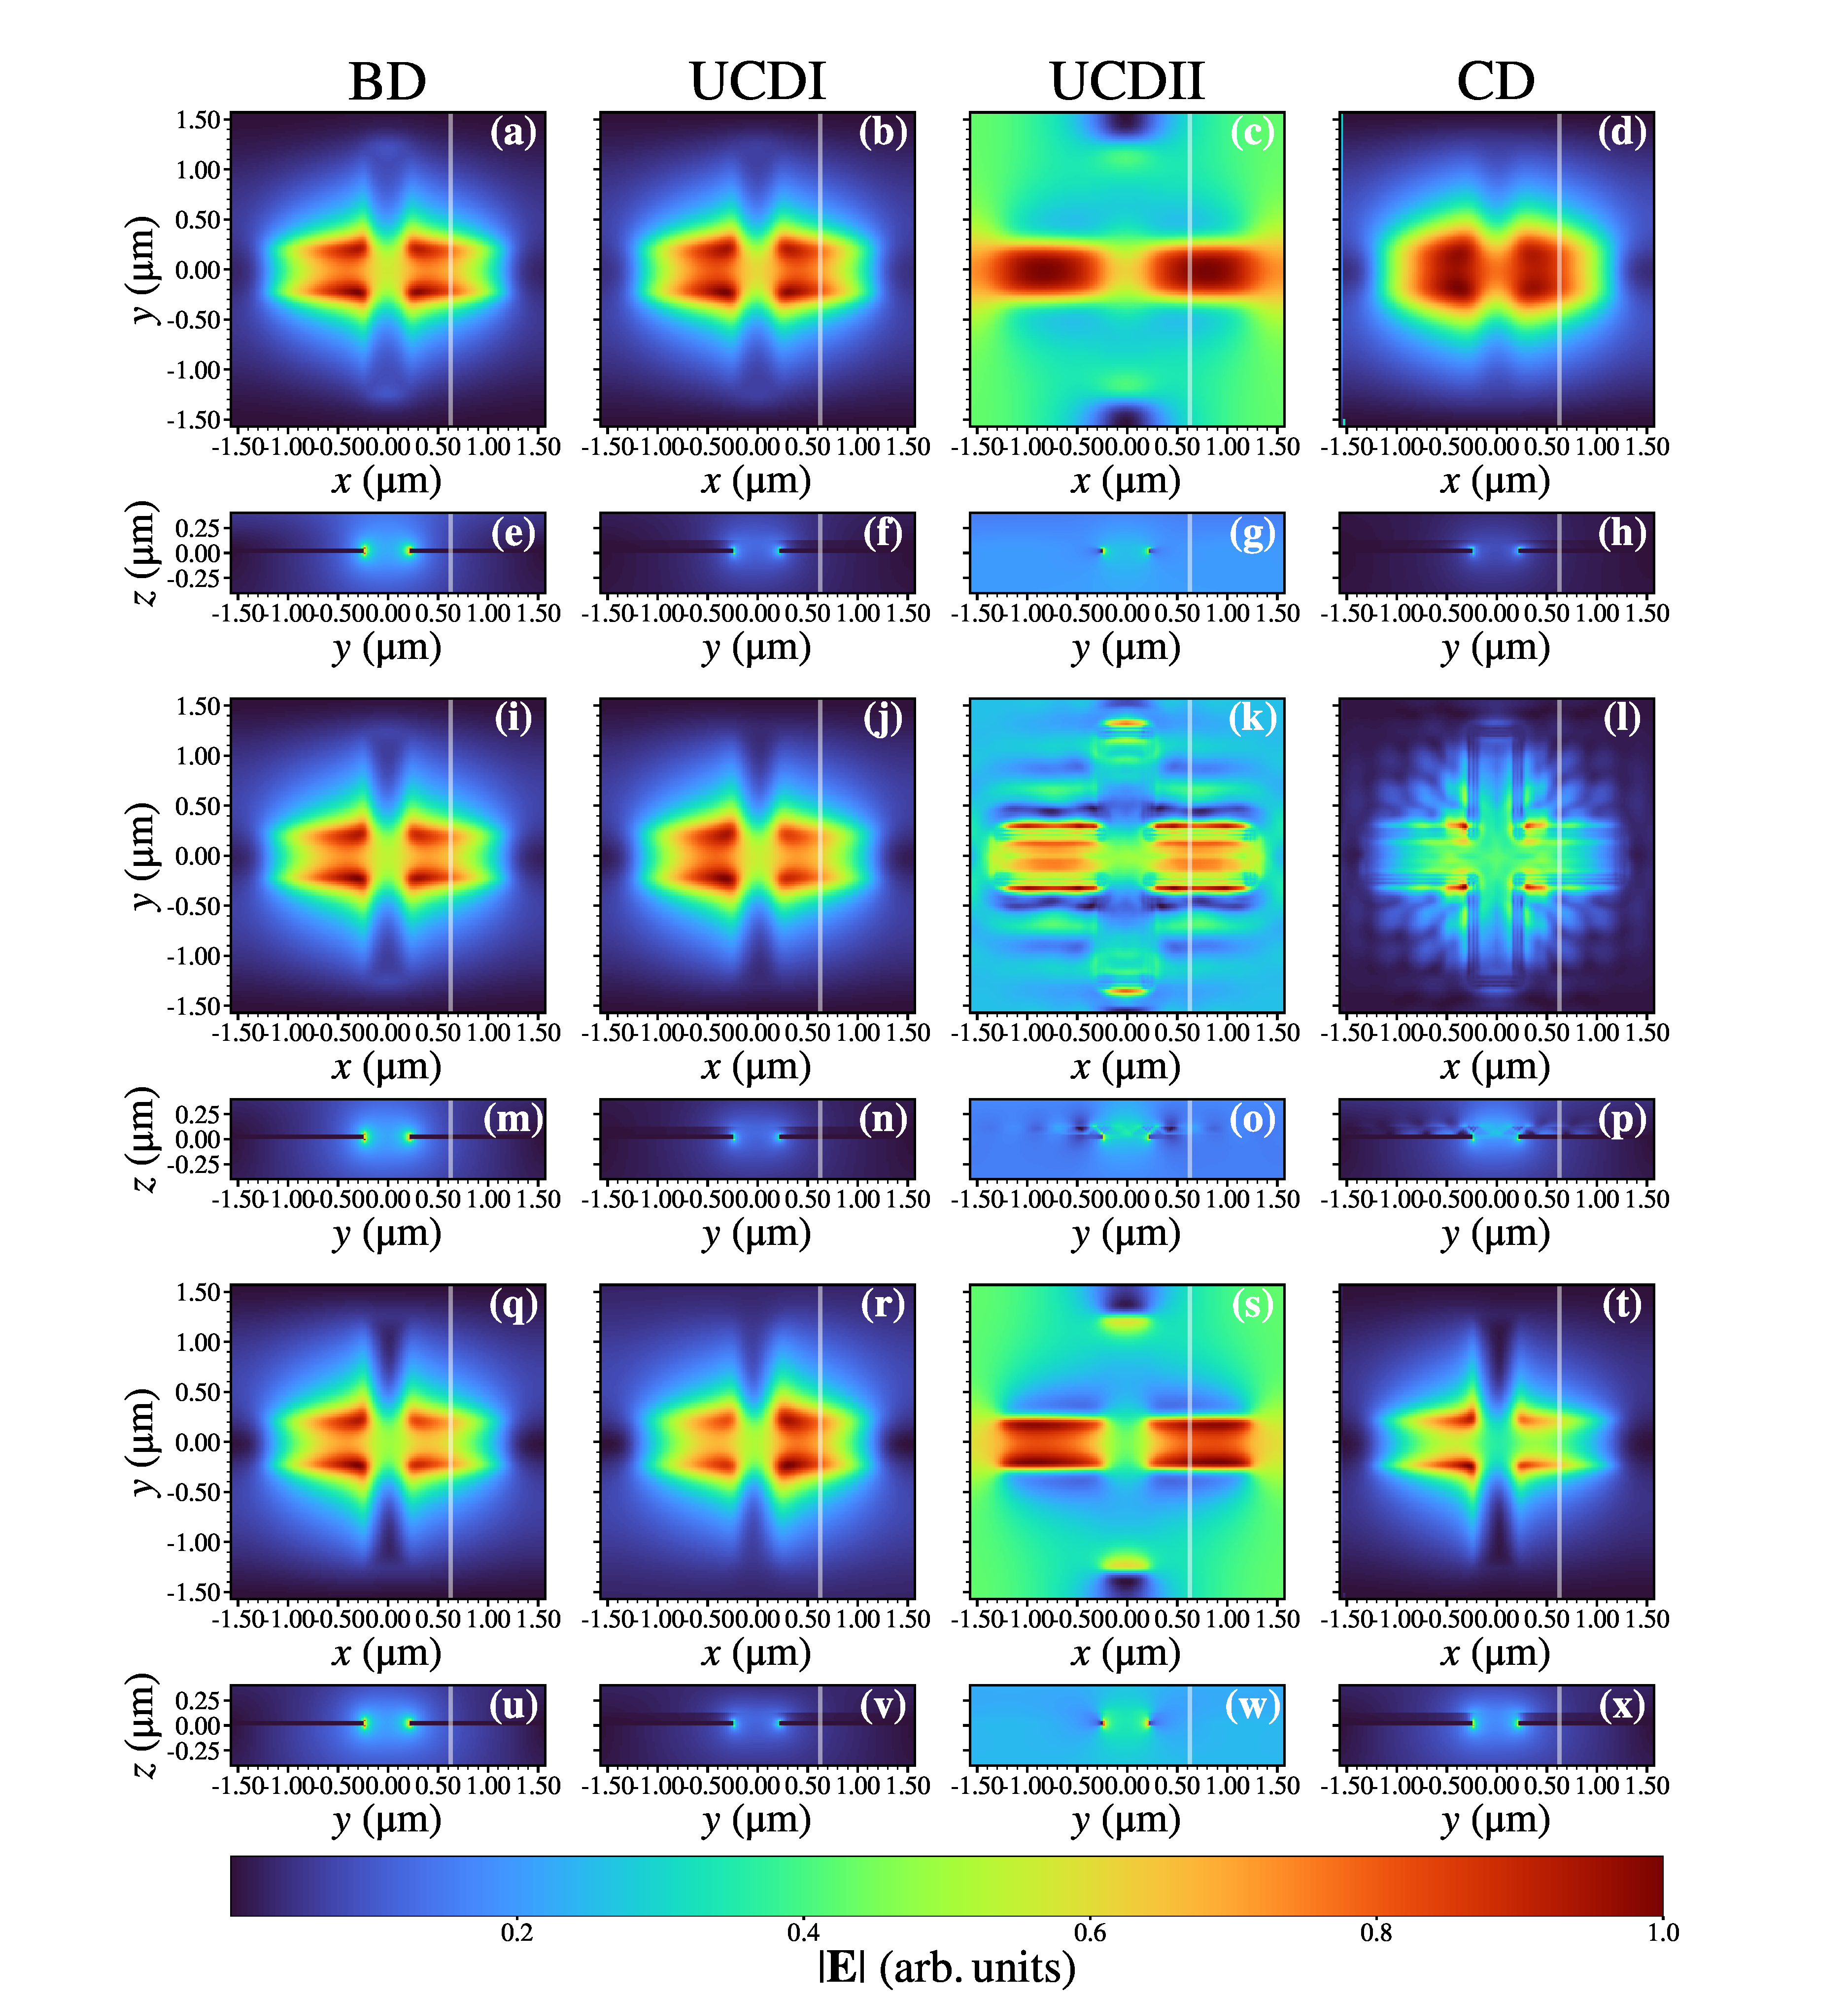
\includegraphics[width=0.95\textwidth]{Mar5DisserrtationPics/Fig4.png}
        % \caption{Rasterized frequency "heat maps" for coupled and uncoupled devices}
        \caption{\textbf{(a)} Absorptance spectra for the uncoupled devices vs the peak frequency of the bare device. The symbols indicate the peak in the absorptance spectra of each uncoupled device and clear show the tuning of the plasmon resonance as function of $d_{CC}$. \textbf{(b)} The absorptance spectra for the hBN (coupled) device. The symbols indicate the peaks in the absorptance spectra and clearly show the coupling between the plasmonic resonance and the hBN TO phonon mode.}
        \label{fig:4}
      \end{figure}

    In order to better analyze the absorptance peak frequency shifts observed in Figure ~\ref{fig:3}, the data in Figure ~\ref{fig:3}(b) and (c) were plotted in colormap form as a function of $\nu_{\rm{bare}}$ in Figure ~\ref{fig:4}(a) and ~\ref{fig:4} (b) respectively. The peak positions were calculated as detailed in the supplemental materials and plotted on top of the colormaps as prescribed in \cite{Wan:16}. Analogously to the reflection data of Wan et al. \cite{Wan:16}, the plasmon peak in the uncoupled device tracks linearly with $\nu_{\rm{bare}}$, while the absorptance peaks of the coupled device open up a small gap and splits into upper and lower branches. For the coupled device with $d_{CC}$ = 2.38 $\rm \mu$m, the difference in frequency between the peaks in absorption is $\Omega$ = 89.7 $\rm cm^{-1}$, which interestingly is close to the range of values, $\Omega$ = 63.4 – 86.7 $\rm cm^{-1}$, reported by Wan et al. for the PMMA/gold meta material structures with PMMA thicknesses ranging from 40 – 100 $\rm \mu$m. Application of degenerate perturbation theory \cite{Sakurai:17} applied to this two-level system enabled the phonon-plasmon coupling strength $\Delta_{PP} = \rm  \Omega = 89.7 cm^{-1}$ to be extracted.

    Figure ~\ref{fig:5} shows components and magnitude of the electric field in a cross-section through center of both the coupled and uncoupled devices with $d_{CC}$  = 2.38 $\rm \mu$m. Data for devices with other values of $d_{CC}$  are presented in the supplemental materials. The fieldmaps shown in Figure ~\ref{fig:5} are four of the frequencies of interest that were monitored within the hBN absorptance peak in Figure  \textcolor{cyan}{ref{fig:2}}(c), namely $\nu$ = 1299, 1361, 1471, and 1538 $\rm cm^{-1}$. By comparing the field maps of the coupled and uncoupled devices, it is possible to isolate the behavior associated with the hBN TO phonon mode. At $\nu$ = 1299 $\rm cm^{-1}$ the field maps for the both the coupled and uncoupled devices are very similar indicating that at this frequency the behavior of the coupled device is predominantly plasmonic. At $\nu$ = 1361 $\rm cm^{-1}$, which is the lowest frequency point of upper branch in Figure ~\ref{fig:5} (b) and is close in frequency to the peak of the hBN in vacuum absorptance band in Figure  \textcolor{cyan}{ref{fig:2}} (c), the data in the coupled device appears to be predominantly plasmonic but the fields are confined in the region of the Ag and hBN layers. At $\nu$ = 1471 $\rm cm^{-1}$, which is in the vicinity of the small fixed frequency absorptance peak in Figure  \textcolor{cyan}{ref{fig:2}} (c), field maps for the both the coupled and uncoupled devices are very different indicating that at this frequency the behavior of the coupled device is predominantly due to the hBN TO phonon. It is notable that in this region the electric field is strongly confined to and appears to be guided within the hBN layer. Finally, at $\nu$ = 1538 $\rm cm^{-1}$, the field maps for both the coupled and uncoupled devices are also very different indicating that at this frequency the behavior of the coupled device is predominantly due to the hBN TO phonon.

    It is not immediately obvious how to extract the polariton wavelength ($\lambda_{P}$) from the above data, in particular the absolute value field data which is directly comparable to experiment. This is due in part not only to the variety and complexity of the mode structure but also due to a non-zero background contribution (see for example, the x-polarized data for the coupled devices in Figure ~\ref{fig:5}). Fortunately, the y-polarized data is comparatively background free showing an alternating field pattern from which the phonon wavelength may be extracted. The y-polarized data was analyzed in the spectral region 1466 – 1570 $\rm cm^{-1}$ and where possible, the distance between successive peaks was averaged (as described in the supplemental materials) in two regions: (a) In the region where the hBN layer was supported by Ag (denoted Vacuum|hBN|Ag) and (b) where the hBN was over one of the circular holes in the Ag film (denoted Vacuum|hBN|Vacuum). In the Vacuum|hBN|Ag case phonon wavelengths in the range $\lambda_{P}$ = 0.16 – 0.33 $\rm \mu$m were extracted. In the Vacuum|hBN|Vacuum case phonon wavelengths in the range $\lambda_{P}$ = 0.40 – 0.70 $\rm \mu$m were extracted. The above values of $\lambda_{P}$ were compared with phonon-polariton dispersion curves calculated using formalism described in [20] for (a) an 80 nm layer of hBN in the Vacuum|hBN|Ag configurationand (b) the Vacuum|hBN|Vacuum configuration. The phonon-polariton wavelengths calculated above were both found to lie close to the expected dispersion curves for the cases (a) and (b) above. There was one notable exception to the data described above. The value of $\lambda_{P}$ = 0.28 $\rm \mu$m for the Vacuum|hBN|Vacuum case monitored at frequencies in the vicinity of $\nu$ = 1466 $\rm cm^{-1}$ was much shorter than expected value of 2.1 $\rm \mu$m indicating that the field variation observed in this case is not solely due to the phonon-polariton, but is caused by some other effect, possibly strong confinement and guiding in the hBN layer.

      \begin{figure}[!htb]
        \centering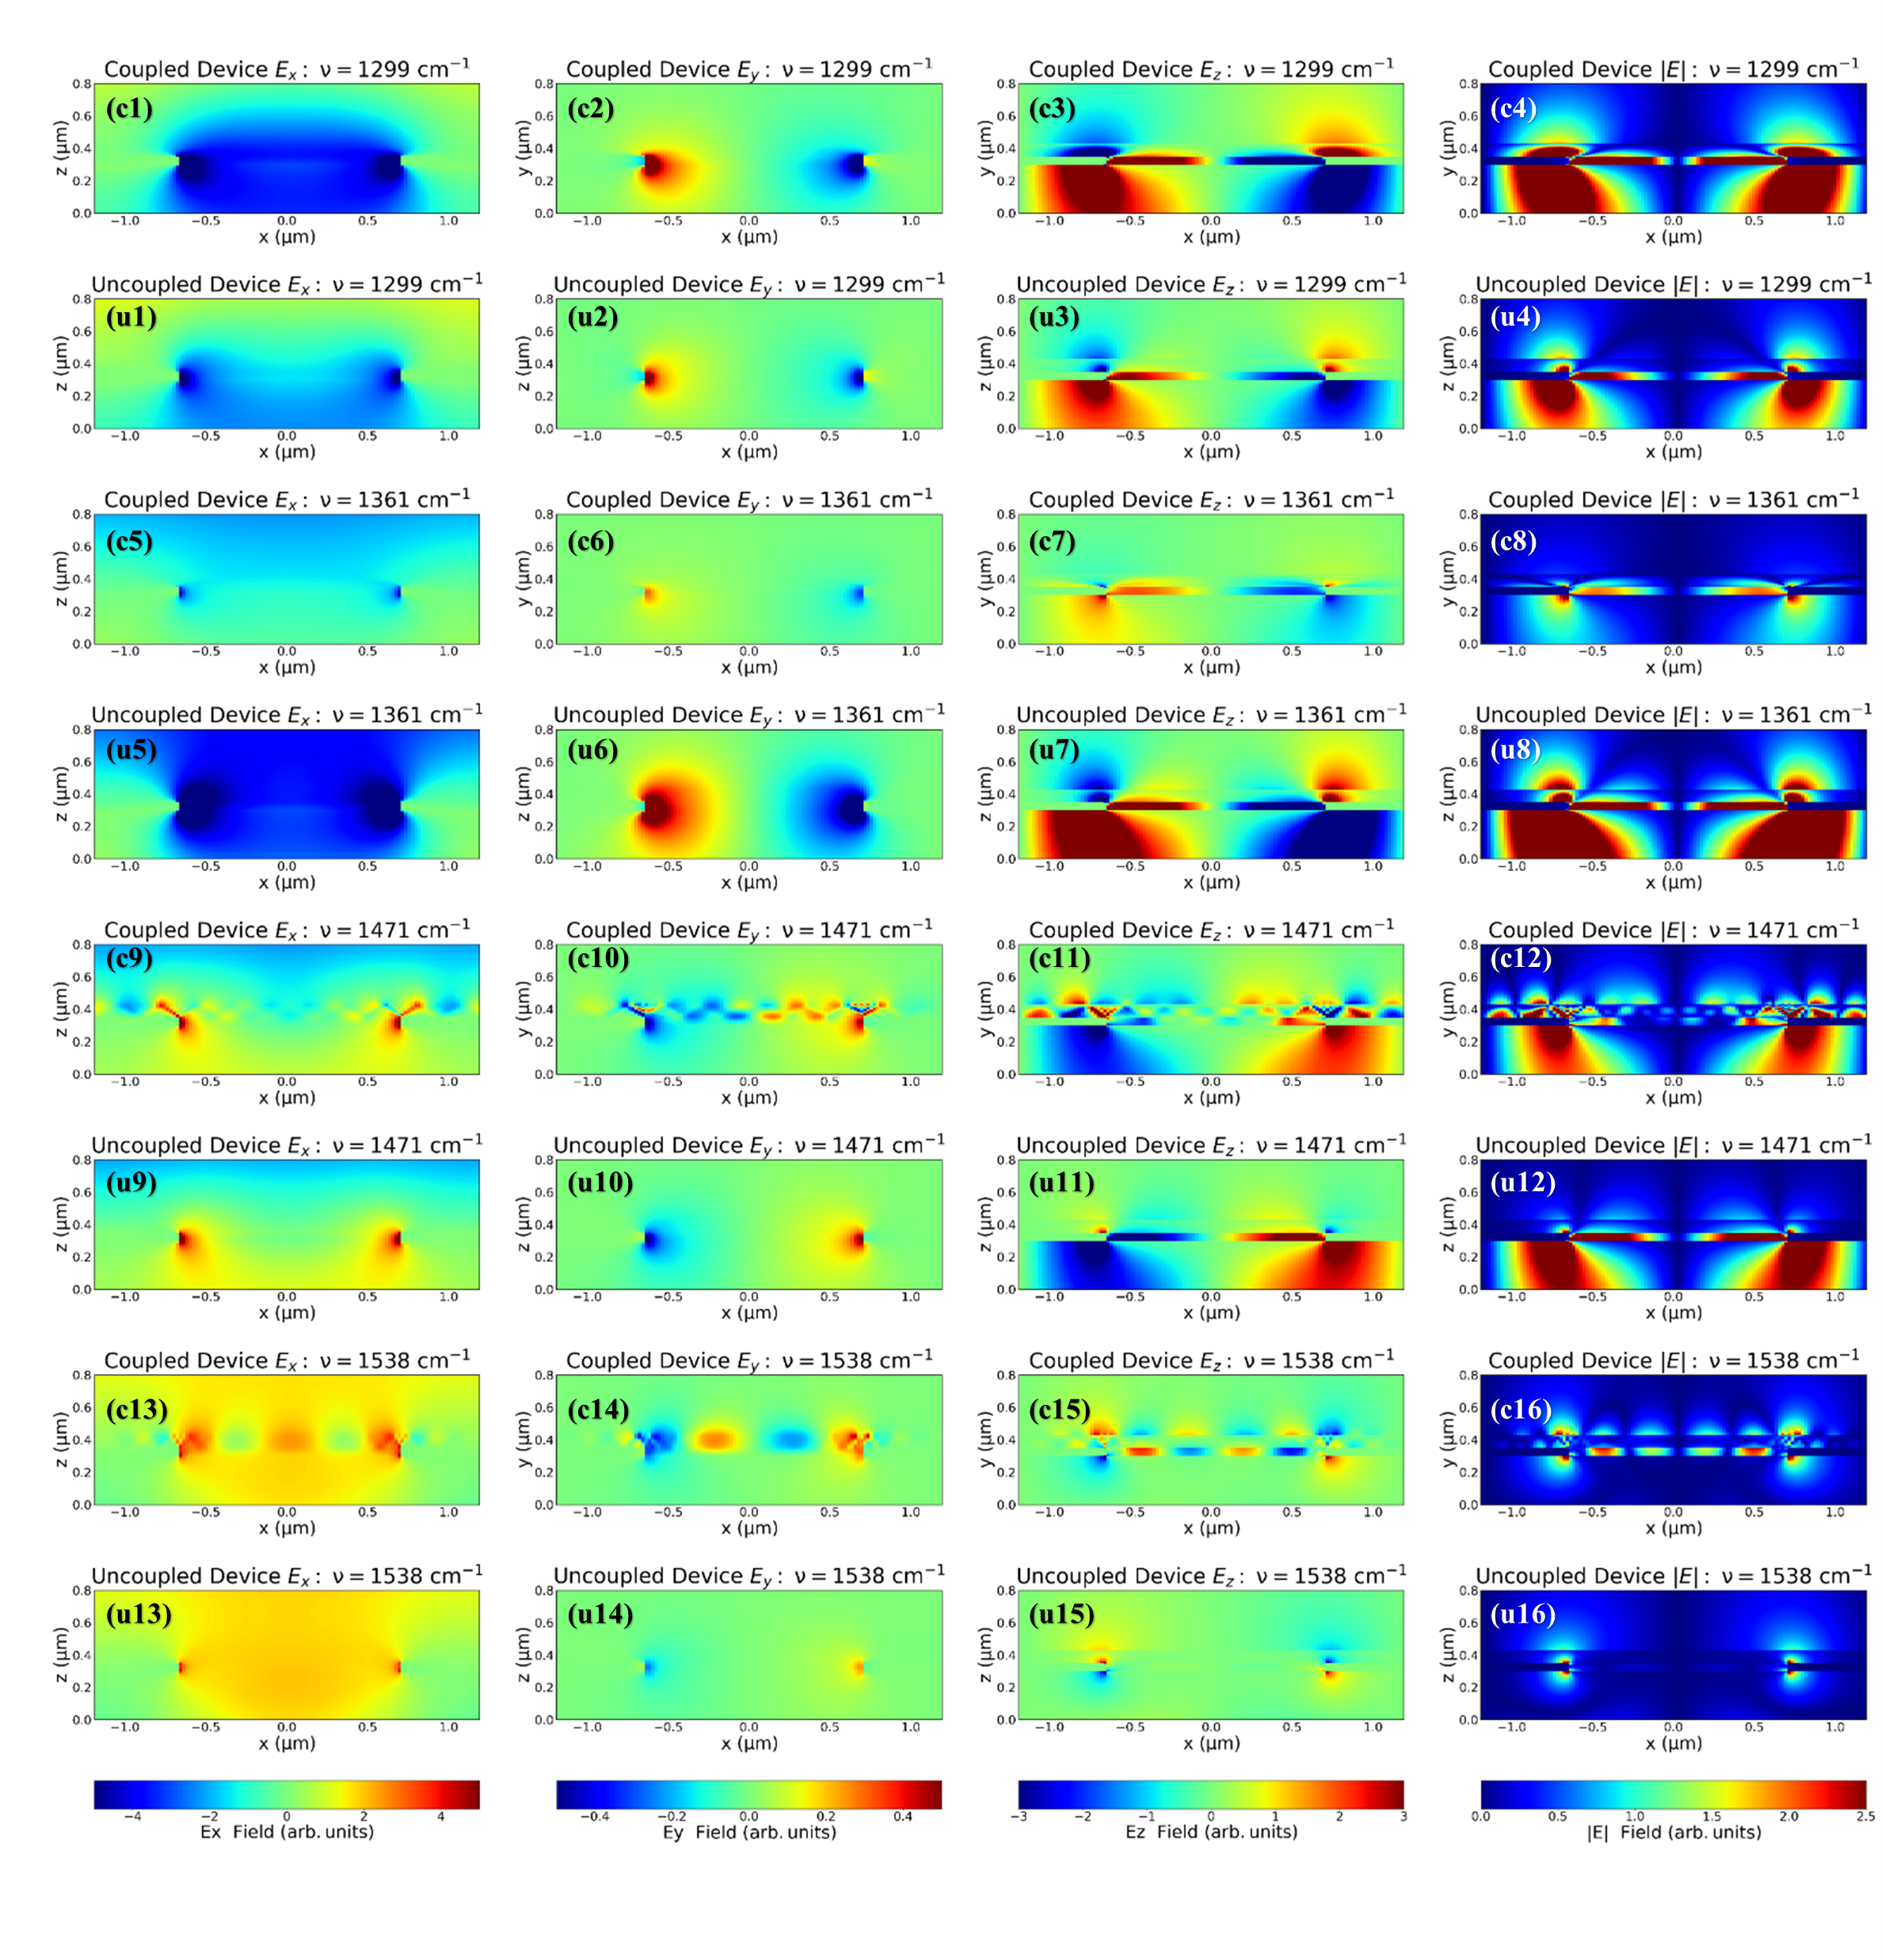
\includegraphics[width=1.0\textwidth]{FiguresCh4/Fig5.png}
        % \caption{Cross-sectional colormaps of the field components in both the hBN (coupled) devices and uncoupled devices at four representative frequencies}
        \caption{Cross-sectional colormaps of the field components in both the hBN (coupled) devices and uncoupled devices at four representative frequencies. Panes \textbf{(c1)}, \textbf{(c2)}, \textbf{(c3)}, and \textbf{(c4)} show the field in the hBN (coupled) device at monitored at 1298 $\rm cm^{-1}$. Panes \textbf{(u1)}, \textbf{(u2)}, \textbf{(u3)}, and \textbf{(u4)} show the field in the uncoupled device at the same frequency. The remaining 16 panes follow the same ordering scheme but for monitoring frequencies of 1361, 1471 and 1538 $\rm cm^{-1}$, respectively.}
        \label{fig:5}
      \end{figure}

      \begin{figure}[!htb]
        \centering\includegraphics[width=0.80\textwidth]{Mar5DisserrtationPics/Fig6Together.png}
        % \caption{Experimental and simulational planar colormaps and their central lineout data.}
        \caption{\textbf{(a)}, \textbf{(b)}, \textbf{(c)}, \textbf{(d)} and \textbf{(e)} Experimental s-SNOM images monitored at 1389, 1408, 1449, 1538 and 1562 $\rm cm^{-1}$, respectively. \textbf{(f)}, \textbf{(g)}, \textbf{(h)}, \textbf{(i)} and \textbf{(j)} Plots of the magnitude if the electric field at the vacuum/hBN interface monitored at 1266, 1408, 1449, and 1538 $\rm cm^{-1}$, respectively. (k) Line-out data from the s-SNOM data plotted as a function of position across the line indicated in \textbf{(a)} - \textbf{(e)}. \textbf{(l)}  Line-out data from the magnitude of the electric field data plotted along the line in \textbf{(f)} - \textbf{(j)}. The dashed lines in \textbf{(l)} and \textbf{(k)} represent the position of the cavity beneath the hBN layer. All data in this figure were individually scaled for greater ease of comparison.}
        \label{fig:6}
      \end{figure}

      Figure ~\ref{fig:6} presents a comparison of s-SNOM data and FDTD electric field ($|\textbf{E}|$) data detected at the hBN/vacuum interface. In an examination of the s-SNOM data and the FDTD field map at 1389 $\rm cm^{-1}$, both show a bright central spot. At 1408 $\rm cm^{-1}$ data show a sharp ring feature within the Ag hole. At 1449 $\rm cm^{-1}$ the ring feature moves further out towards the edge of the Ag hole. At 1538 $\rm cm^{-1}$, there is a slow variation within the Ag hole with a weaker maximum at the center, while outside the Ag hole fine fringes can be observed which are attributed to phonon-polaritons. Finally, at 1562 $\rm cm^{-1}$, the fringes inside the Ag hole move further toward the edge of the. Outside the Ag hole fine fringes can still be observed, although they are weaker than those observed in the 1538 $\rm cm^{-1}$ case. The above behavior can also be observed by comparing the line-out data in Figure ~\ref{fig:6} (k) and (l).
  \section{Conclusion}
  \label{sec:conclusion}
    The excitations that occur on a hBN/nanopatterened Ag device have been investigated using a combination of experimental (s-SNOM) and simulational (FDTD) techniques. The s-SNOM data shows high spatial frequency features when the structure is excited in the region 1370 –1590 $\rm cm^{-1}$  and predominantly low spatial frequency features when excited outside of the spectral region. FDTD simulations of a model structure exhibit similar behavior. In addition, an examination of absorption spectra for the device indicates that the degenerate phonon and plasmon peaks split and shift enabling the phonon-plasmon coupling strength to be estimated, \textit{i.e.}, $\Delta{\rm{PP}}$ = 89.7 $\rm cm^{-1}$  to be made. Access to the individual field component afforded by the FDTD simulations enabled the polariton wavelength as function of frequency to be extracted. The results presented in this paper therefore contribute to a deeper and more fundamental understanding of the interactions between phonons and plasmons in this and related structures and devices.

\bibliography{hBNPaper.bib}
\end{document}		